\documentclass[12pt]{report}
\usepackage{geometry}
\usepackage{setspace}
\usepackage{lipsum}
\usepackage{graphicx}
\usepackage{caption}
\geometry{a4paper, left=3cm, right=2cm, top=2.5cm, bottom=2.5cm}
\graphicspath{{figures/}}
\begin{document}

\begin{titlepage}
    \begin{center}
        \vspace*{1cm}
        
        \textbf{\large DETERMINANTS OF ENVIRONMENTAL DEPENDENCY: \\ CASE OF MOUNTAIN, MID-HILL AND LOWLAND REGION ON NEPAL}
        
        \vspace{1.5cm}
        
        \textbf{ A THESIS} \\
        
        \textbf{SUBMITTED TO THE \\
        CENTRAL DEPARTMENT OF ECONOMICS, \\
        FACULTY OF HUMANITIES AND SOCIAL SCIENCES, \\
        TRIBHUVAN UNIVERSITY.}
        
        \vspace{1.5cm}
        
        \textbf{IN PARTIAL FULFILLMENT OF THE REQUIREMENTS FOR THE \\
        MASTER DEGREE OF ARTS \\
        IN \\
        ECONOMICS.}
        
        \vspace{1.5cm}
        
        \textbf{BY \\
        SANJEEV NHEMHAFUKI \\
        ROLL NO: 51/076 \\
        TU REGISTRATION NO: 7-2-32-90-2013}
        
        \vspace{1.5cm}
        
        \textbf{CENTRAL DEPARTMENT OF ECONOMICS \\
        TRIBHUVAN UNIVERSITY \\
        KIRTIPUR, KATHMANDU, NEPAL.}
        
        \vspace{1.5cm}
        
        \textbf{DECEMBER, 2023}
        
    \end{center}
\end{titlepage}

\newpage % Start content on a new page
\begin{center}
\section*{DECLARATION}
\end{center}
\addcontentsline{toc}{section}{Declaration}
\renewcommand{\thepage}{\roman{page}}
\setcounter{page}{1}
\setstretch{1.5} % Line-spacing betwenen the lines
This thesis entitled, “DETERMINANTS OF ENVIRONMENTAL DEPENDENCY: CASE OF MOUNTAIN, MID-HILL AND LOWLAND REGION ON NEPAL”, was conducted under the supervision of Associate Professor Resham B. Thapa, PhD of Central Department of Economics, Tribhuvan University. I declare that the results and analysis reported in this thesis is the result of my own study, except where due reference has been made. The thesis has not been accepted for any degree nor has been submitted for candidature in other degree granting programs.

\vspace{2cm}

\begin{flushright}
    ................................\\
    Date: December 30, 2023 A.D. \ \ \ \ \ \ \ \ \ \ \ \ \ \ \ \ \ \ \ \ \ \ \ \ \ \ \ \ \ \  \ \ \ \ \ \ \ \ \ \ \ \ \ \ \ \ \ \ \ \ \ \ \ \  Sanjeev Nhemhafuki\\
    TU Reg. No: 7-2-32-90-2013
\end{flushright}

\newpage % Start content on a new page
\begin{center}
\section*{LETTER OF RECOMMENDATION}
\end{center}
\addcontentsline{toc}{section}{Letter of Recommendation}
\renewcommand{\thepage}{\roman{page}}
\setcounter{page}{2}
\setstretch{1.5}
This thesis entitled,“DETERMINANTS OF ENVIRONMENTAL DEPENDENCY: CASE OF MOUNTAIN, MID-HILL AND LOWLAND REGION ON NEPAL”, is submitted by Mr. Sanjeev Nhemhafuki under my supervision for partial fulfillment of the requirements for the degree of MASTER OF ARTS in ECONOMICS. I forward it with a recommendation for approval.

\vspace{2cm}

\begin{flushright}
    ................................\\
    Date: December 30, 2023 A.D. \ \ \ \ \ \ \ \ \ \ \ \ \ \ \ \ \ \ \ \ \ \ \ \ \ \ \ \ \ \ \ \ \ \ \ \ \ \ \ \ \ \ \  \ \ \ \ \ \ \ \ \ \ \ \ \ \ \ \ \ \ \ \ \ \ \ \  Resham Thapa-Parajuli, PhD\\
    Thesis Supervisor
\end{flushright}

\newpage % Start content on a new page
\begin{center}
\section*{APPROVAL LETTER}
\end{center}
\addcontentsline{toc}{section}{Approval Letter}
\renewcommand{\thepage}{\roman{page}}
\setcounter{page}{3}
\setstretch{1.5}
We certify that this thesis entitled, “DETERMINANTS OF ENVIRONMENTAL DEPENDENCY: CASE OF MOUNTAIN, MID-HILL AND LOWLAND REGION ON NEPAL” submitted by Mr. Sanjeev Nhemhafuki to the Central Department of Economics, Faculty of Humanities and Social Sciences, Tribhuvan University, in the partial fulfillment of the requirement for the  MASTER OF ARTS in ECONOMICS has been found satisfactory in scope and quality. Therefore, we accept this thesis as a part of the said degree.
\vspace{2cm}

\begin{flushright}
Thesis Committee 
\vspace{1cm} \\
    ................................\\
Prof. Shiva Raj Adhikari, PhD \\
 Head of the Department 
\vspace{1cm} \\
................................\\
Professor \\
External Examiner 
\vspace{1cm} \\
................................\\
 Date: December 30, 2023 A.D. \ \ \ \ \ \ \ \ \ \ \ \ \ \ \ \ \ \ \ \ \ \ \ \ \ \ \ \ \ \ \ \ \ \ \ \ \ \ \ \ \ \ \  \ \ \ \ \ \ \ \ \ \ \ \ \ \ \ \ \ \ \ \ \   ReshamThapa-Parajuli, PhD\\
    Thesis Supervisor

\end{flushright}
\newpage % Start content on a new page
\begin{center}
\section*{ACKNOWLEDGEMENTS}
\end{center}
\addcontentsline{toc}{section}{Acknowledgements}
\renewcommand{\thepage}{\roman{page}}
\setcounter{page}{4}
\setstretch{1.5}
I would to convey my gratitude for all of the support and guidance that the faculty and CEDECON staff provided to me during my in CEDECON. Firstly, I would like to express sincere thanks to Asst. Prof. Mr. Resham B. Thapa, PhD, for his unwavering support and insightful mentoring. He has consistently inspired me, and I am incredibly appreciative of his input in finishing this thesis. I express my gratitude to the department head, Prof. Dr. Shiva Raj Adhikari, for his thoughtful advice and academic guidance. 

My appreciation goes along to Assistant Professor Naveen Adhikari, Associate Professor Nirmal K. Raut, Assistant Professor Khagendra Katuwal, and all of the other distinguished faculty members and personnel at CEDECON. Their  presence in CEDECON have been invaluable to my studies, and I acknowledge all of their hard work and encouragement. I am grateful of the opportunities and resources the department provided to me during my studies. 

I am thankful to Manab Prakash Poudel, Subin K.C, Shreezal G.C, Sanjit Singh Thapa, Mohan Khanal, Hemant Panthi, Tilak C. Kshetri for inspiring and motivating me to read and write. I would like to thank my friends Roja Pradhanaga, Sita Malla Thakuri, Kishor Gosai, Rojina Banmala, Bhawana Basnet, for their kindness and for making my stay in Kirtipur wonderful. My academic experience has been enhanced by their friendship and collaboration, and I am pleased for the opportunity I got to learn alongside them.

Finally, I would like to thank my family for their love and support. They have consistently encouraged me to give my best, and I am grateful of continuous backing. I'm grateful for everything, everyone. I am appreciative of all of your advice and assistance.

\vspace{1cm}

\begin{flushright}

 Date: December 30, 2023 A.D. \ \ \ \ \ \ \ \ \ \ \ \ \ \ \ \ \ \ \ \ \ \ \ \ \ \ \ \  \ \ \ \ \ \ \ \ \ \ \ \ \ \ \ \ \ \ \ \ \ \ Sanjeev Nhemhafuki\\
    Bhaktapur

\end{flushright}

\newpage % Start content on a new page
\begin{center}
\section*{ABSTRACT}
\end{center}
\addcontentsline{toc}{section}{Abstract}
\renewcommand{\thepage}{\roman{page}}
\setcounter{page}{5}
\setstretch{1.5}


\vspace{2cm}

\begin{flushright}


\end{flushright}

\newpage
\tableofcontents
% Content for Declaration

\clearpage % Start content on a new page
\begin{center}
\section*{LIST OF TABLES}
\end{center}
\addcontentsline{toc}{section}{List of Tables}
\renewcommand{\thepage}{\roman{page}}
\setcounter{page}{6}
\setstretch{1.5}


\vspace{2cm}


\newpage % Start content on a new page
\begin{center}
\section*{LIST OF FIGURES}
\end{center}
\addcontentsline{toc}{section}{List of Figures}
\renewcommand{\thepage}{\roman{page}}
\setcounter{page}{7}
\setstretch{1.5}


\vspace{2cm}

\newpage % Start content on a new page
\begin{center}
\section*{LIST OF ABBREVIATIONS}
\end{center}
\addcontentsline{toc}{section}{List of Abbreviations}
\renewcommand{\thepage}{\roman{page}}
\setcounter{page}{8}
\setstretch{1.5}


\vspace{2cm}


\clearpage % Start content on a new page
\begin{center}
\section*{CHAPTER I \\ INTRODUCTION}
\end{center}
\addcontentsline{toc}{section}{CHAPTER I  INTRODUCTION}
\renewcommand{\thepage}{\arabic{page}}

\setstretch{1.5}


\vspace{2cm}


\subsection*{1.1 Introduction}
\addcontentsline{toc}{subsection}{1.1 Introduction}
\renewcommand{\thepage}{\arabic{page}}

\setstretch{1.5}
\vspace{2cm}


\subsection*{1.2 Statement of the Problem }
\addcontentsline{toc}{subsection}{1.2 Statement of the Problem }
\renewcommand{\thepage}{\arabic{page}}
\setcounter{page}{1}
\setstretch{1.5}
\vspace{2cm}


\subsection*{1.3 Research questions}
\addcontentsline{toc}{subsection}{1.3 Research questions }
\renewcommand{\thepage}{\arabic{page}}

\setstretch{1.5}
\vspace{2cm}

\subsection*{1.4 Objectives }
\addcontentsline{toc}{subsection}{1.4 Objectives  }
\renewcommand{\thepage}{\arabic{page}}

\setstretch{1.5}

\textbf{General Objectives}
\\
\textbf{Specific Objectives}
\vspace{2cm}


\subsection*{1.5 Significance of the Study}
\addcontentsline{toc}{subsection}{1.5 Significance of the Study}
\renewcommand{\thepage}{\arabic{page}}

\setstretch{1.5}
\vspace{2cm}

\subsection*{1.6 Scope and Limitations of the study}
\addcontentsline{toc}{subsection}{1.6 Scope and Limitations of the study}
\renewcommand{\thepage}{\arabic{page}}

\setstretch{1.5}
\vspace{2cm}

\subsection*{1.7 Organizations of the study}
\addcontentsline{toc}{subsection}{1.7 Organizations of the study}
\renewcommand{\thepage}{\arabic{page}}

\setstretch{1.5}
\vspace{2cm}

\clearpage

\begin{center}
\section*{CHAPTER II \\ REVIEW OF LITERATURE }
\end{center}
\addcontentsline{toc}{section}{CHAPTER II REVIEW OF LITERATURE }
\renewcommand{\thepage}{\arabic{page}}
\setcounter{page}{3}
\setstretch{1.5}
\vspace{2cm}


\subsection*{2.1  Introduction}
\addcontentsline{toc}{subsection}{2.1 Introduction}
\renewcommand{\thepage}{\arabic{page}}

\setstretch{1.5}
\vspace{2cm}


\subsection*{2.2 Origin and development of informality}
\addcontentsline{toc}{subsection}{2.2 Origin and development of informality}
\renewcommand{\thepage}{\arabic{page}}

\setstretch{1.5}
\vspace{2cm}


\subsection*{2.3 Environmental Dependency and Social Vulnerability}
\addcontentsline{toc}{subsection}{2.3 Environmental Dependency and Social Vulnerability}
\renewcommand{\thepage}{\arabic{page}}

\setstretch{1.5}
\vspace{2cm}

\subsection*{2.4 Empirical reviews}
\addcontentsline{toc}{subsection}{2.4 Empirical reviews}
\renewcommand{\thepage}{\arabic{page}}
\setstretch{1.5}

\vspace{2cm}


\subsection*{2.5 Review of national studies}
\addcontentsline{toc}{subsection}{2.5 Review of national studies}
\renewcommand{\thepage}{\arabic{page}}

\setstretch{1.5}
\vspace{2cm}

\subsection*{2.6 Research gap}
\addcontentsline{toc}{subsection}{2.6 Research gap}
\renewcommand{\thepage}{\arabic{page}}

\setstretch{1.5}
\vspace{2cm}


\clearpage
\begin{center}
\section*{CHAPTER III \\ RESEARCH METHODOLOGY }
\end{center}
\addcontentsline{toc}{section}{CHAPTER III RESEARCH METHODOLOGY }
\renewcommand{\thepage}{\arabic{page}}
\setcounter{page}{4}
\setstretch{1.3}
\vspace{1cm}
This section discusses the theoretical and conceptual framework of the study. Sustainable rural livelihood framework proposed by  DfID (1999b) and Household Vulnerability assessment framework approach is used to examine the Household vulnerability. The following sections describes the sample design, conceptual frame work , sources of data and techniques for data analysis. \par
\vspace{1cm}
\subsection*{3.1  Philosophical Issues}
\addcontentsline{toc}{subsection}{3.1  Philosophical Issues}
\renewcommand{\thepage}{\arabic{page}}

\setstretch{1.3}
This study adopts a research paradigm influenced by radical structuralism, which assumes that household vulnerability is objectively determined by factors such as Social Asset, Human Asset, Natural Asset, Financial Asset, and Physical Asset. The ontological position of this study is objectivism, as it aims to produce objective and value-free knowledge about reality as a part of economics research. The epistemological position is positivism, as it relies on empirical methods and data to develop and test theories Household Vulnerability. The axiological position is value-free, as the researcher endeavors to not be influenced by or influence the subject or results of the study. The philosophical tradition that guides this study is the Neo-classical framework.\par

\graphicspath{{figures/}}
\begin{figure}[h]
    \centering
    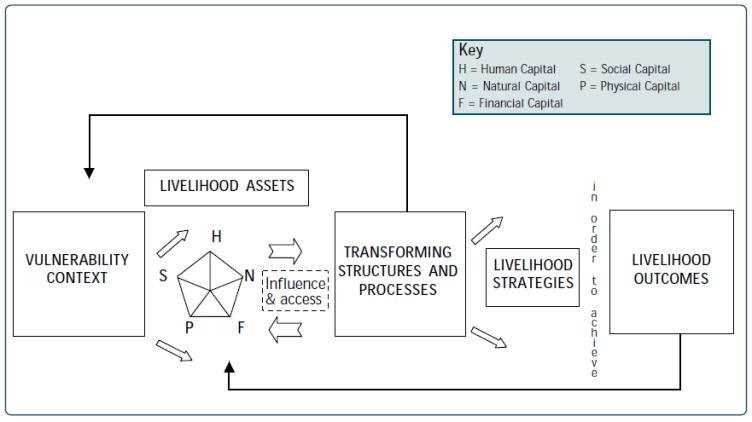
\includegraphics[scale=0.5]{DFID Rural livelihood approach.png}
    \caption*{Figure 3.1: Conceptual Framework of the Study adapted from} \cite(dfid1999sustainable)
    \label{fig:conceptualfw}
\end{figure}
\subsection*{3.2 Research design}
\addcontentsline{toc}{subsection}{3.2 Research design}
\renewcommand{\thepage}{\arabic{page}}
\setcounter{page}{1}
\setstretch{1.5}
\vspace{2cm}


\subsection*{3.3 Conceptual framework}
\addcontentsline{toc}{subsection}{3.3 Conceptual framework}
\renewcommand{\thepage}{\arabic{page}}

\setstretch{1.5}
\vspace{2cm}

\subsection*{3.4 Sources of data}
\addcontentsline{toc}{subsection}{3.4 Sources of data}
\renewcommand{\thepage}{\arabic{page}}
\setstretch{1.5}

\vspace{2cm}

\subsubsection{3.4.1. Secondary data}
\addcontentsline{toc}{subsection}{\ \ \ \ \ 3.4.1 Secondary data}
\renewcommand{\thepage}{\arabic{page}}
\setstretch{1.5}

\vspace{2cm}

\subsection*{3.5 Techniques of Data Analysis}
\addcontentsline{toc}{subsection}{3.5 Techniques of Data Analysis}
\renewcommand{\thepage}{\arabic{page}}
\setstretch{1.5}


\clearpage
\begin{center}
\section*{CHAPTER IV \\  RESULTS AND DISCUSSION }
\end{center}
\addcontentsline{toc}{section}{CHAPTER IV  RESULTS AND DISCUSSION }
\renewcommand{\thepage}{\arabic{page}}
\setcounter{page}{5}
\setstretch{1.5}
\vspace{2cm}


\subsection*{4.1 Descriptive Statistics}
\addcontentsline{toc}{subsection}{4.1   Descriptive Statistics}
\renewcommand{\thepage}{\arabic{page}}

\setstretch{1.5}
\vspace{2cm}

\subsection*{4.2 Discussion}
\addcontentsline{toc}{subsection}{4.2 Discussion}
\renewcommand{\thepage}{\arabic{page}}
\setstretch{1.5}

\clearpage
\clearpage
\begin{center}
\section*{CHAPTER V \\  CONCLUSION AND RECOMMENDATIONS }
\end{center}
\addcontentsline{toc}{section}{CHAPTER V  CONCLUSION AND RECOMMENDATIONS }
\renewcommand{\thepage}{\arabic{page}}
\setcounter{page}{6}
\setstretch{1.5}
\vspace{2cm}


\subsection*{5.1 Conclusion}
\addcontentsline{toc}{subsection}{5.1 Conclusion}
\renewcommand{\thepage}{\arabic{page}}

\setstretch{1.5}
\vspace{2cm}

\subsection*{5.2 Discussion}
\addcontentsline{toc}{subsection}{5.2 Recommendations}
\renewcommand{\thepage}{\arabic{page}}
\setstretch{1.5}

\subsection*{5.3  Possible extension}
\addcontentsline{toc}{subsection}{5.3  Possible extension}
\renewcommand{\thepage}{\arabic{page}}
\setstretch{1.5}
\end{document}
